% !TeX root = ../../thesis.tex
\chapter{Top-Illuminated Photodiodes for CMOS Integration}\label{ch:top_illuminated}

\section{Comparison Between Silicon and Glass Substrate}

So far, we have established as the baseline stack the one deposited with a total deposition rate of 0.8{\AA}/s, at a stoichiometry of 1.05:1.00 CsBr:\ch{PbI_2}, with 40 nm of \ch{TiO_2} as the ETL. At this point we can transfer the same stack to the silicon substrates (Fig.~\ref{fig:ch2:pix_stack}). 
The device on silicon substrate exhibits significantly higher hysteresis and lower rectification, mainly attributed to the higher resistance of the TiN contact. In terms of the device's EQE, a significantly lower response at 0 V compared to the glass substrate. When increasing the bias to -1 V, it is possible to saturate, again. The slow turn-on of the diode is more explicitly illustrated at the EQE as a function of bias. 



\begin{figure}[htbp]
    \centering
    \begin{subfigure}{0.32\textwidth}
        \centering
        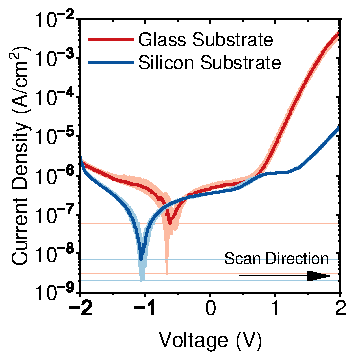
\includegraphics[width=\textwidth]{chapters/material_properties/images/JV_PIX_Glass.pdf}
        \caption{}
        \label{fig:ch2:jv_comp_pic_glass}
    \end{subfigure}
    \hfill
    \begin{subfigure}{0.32\textwidth}
        \centering
        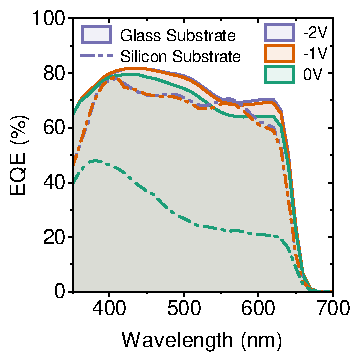
\includegraphics[width=\textwidth]{chapters/material_properties/images/EQE_fnm_PIX_Glass.pdf}
        \caption{}
        \label{fig:ch2:eqe_comp_pix_glass}
    \end{subfigure}
    \hfill
    \begin{subfigure}{0.32\textwidth}
        \centering
        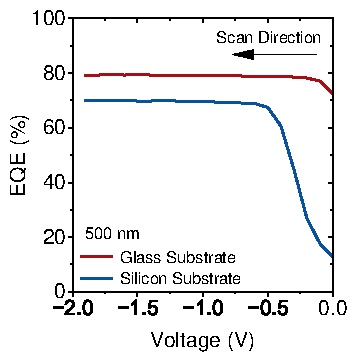
\includegraphics[width=\textwidth]{chapters/material_properties/images/EQE_fV_PIX_Glass.pdf}
        \caption{}
        \label{fig:plot3}
    \end{subfigure}
    
    \caption{A 1×3 grid of images.}
    \label{fig:ch2:eqefV_comp_pix_glass}
\end{figure}


Two potential causes could be evaluated for the slower turn-on of the diode when it is fabricated on top of the Si substrate. In contrast to ITO and Al that were used as contacts for the glass substrate, which have a large difference in the work function, ITO and TiN do not have a big difference in their work function. To further evaluate this, we fabricate the same stack on glass substrate, using ITO as top and bottom contact. In this case, it is clear that EQE saturates, indicating that the built-in potential is sufficient to fully extract the generated carriers, even at 0 V. Therefore, we turn to the second possible reason that could cause the slower turn-on of the diode, and that is the potential existence of an energy barrier. To investigate this we turn to the substrate itself and the interface between TiN and \ch{NiO_x}. We submit four different substrates to TEM, one that is as-deposited, and the rest annealed in open air at 300 \degree C for 5 minutes, 30 minutes, and 60 minutes, respectively. The results are illustrated in Fig.~\ref{fig:ch2:tem_pix_substrate}. For all samples, even for the as-deposited one, a thin layer of \ch{TiO_2} is observed. Additionally, the following trend is observed: with increasing annealing duration, the thickness of the \ch{TiO_x} layer remains the same, however the levels of oxygen are increasing. TiOx could introduce an energy barrier, that is preventing the extraction of carriers at 0 V.

\begin{figure}[htbp]
    \centering
    % First row
    \begin{subfigure}[t]{0.49\textwidth}
        \centering
        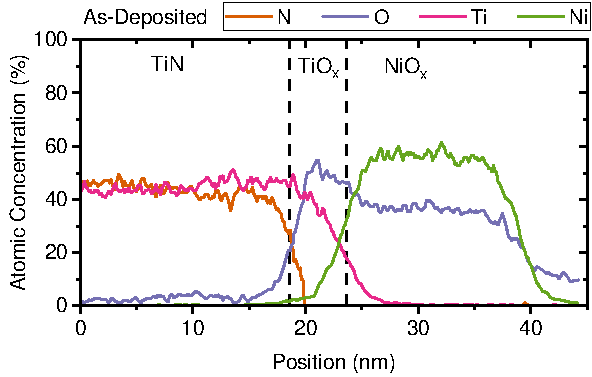
\includegraphics[width=\textwidth]{chapters/material_properties/images/TEM_As_Dep.pdf} % Replace with your image file
        \caption*{(a)}
    \end{subfigure}
    \hfill
    \begin{subfigure}[t]{0.49\textwidth}
        \centering
        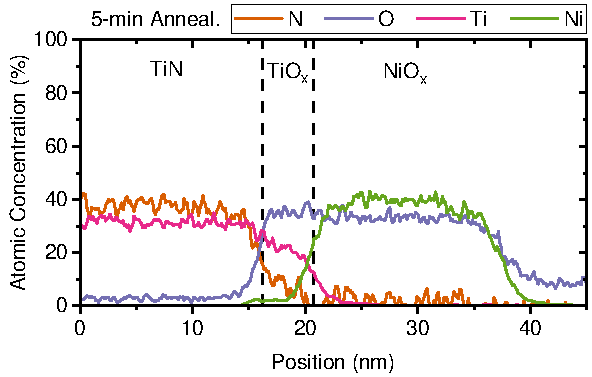
\includegraphics[width=\textwidth]{chapters/material_properties/images/TEM_5_min.pdf} % Replace with your image file
        \caption*{(b)}
    \end{subfigure}


    % Second row
    \begin{subfigure}[t]{0.49\textwidth}
        \centering
        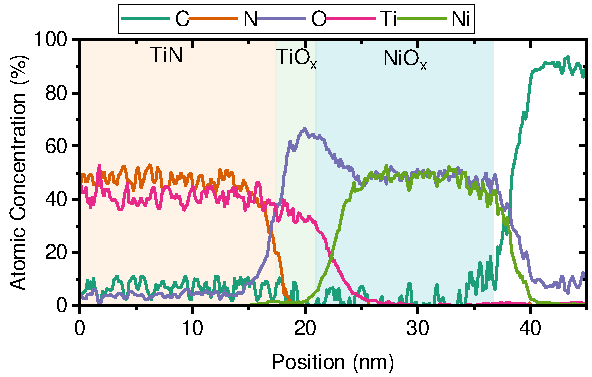
\includegraphics[width=\textwidth]{chapters/material_properties/images/TEM_30_min.pdf} % Replace with your image file
        \caption*{(c)}
    \end{subfigure}
    \hfill
    \begin{subfigure}[t]{0.49\textwidth}
        \centering
        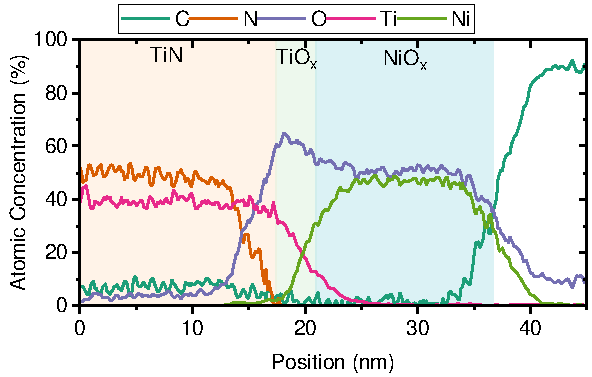
\includegraphics[width=\textwidth]{chapters/material_properties/images/TEM_60_min.pdf} % Replace with your image file
        \caption*{(d)}
    \end{subfigure}
    \caption{TEM of TiN - NiOx interface and emergence of TiOx at the interface.}
    \label{fig:ch2:tem_pix_substrate}
\end{figure}



\section{High-Temperature Performance}




%%%%%%%%%%%%%%%%%%%%%%%%%%%%%%%%%%%%%%%%%%%%%%%%%%
% Keep the following \cleardoublepage at the end of this file, 
% otherwise \includeonly includes empty pages.
\cleardoublepage

